\chapter{TO be checked what can be deleted or kept in other sections}
    \section{Frame}
        The choice of the drone frame is really important. The size of the frame will impact the choice of the propellers, the motors, the \acrshort{esc} and the battery. It has to be big enough to have enough space for all the components of the drone.
        
        As the aim is to create a swarm of drone, the smaller the frame is the better.
        
        The most stringent requirement for the choice of the frame is to fit the \gls{oc}. So, I choose the smallest size of frame that could fit the \gls{oc} and have propellers commonly used for this size. So, it was a 330mm frame with 7 inch propeller to have a hub diameter of 152mm \ref{fig:330_7} (enough to fit the \gls{oc}). But this size was to large, so a smaller was chosen at the cost of smaller propeller. The efficiency  is reduced as the propeller need to rotate faster which mean higher \gls{kv}. So, a size of 275mm frame with 5 inch propeller was choosen with a hub diameter of 148mm \ref{fig:275_5.png}.
        
        \begin{figure}[!ht]
            \centering
            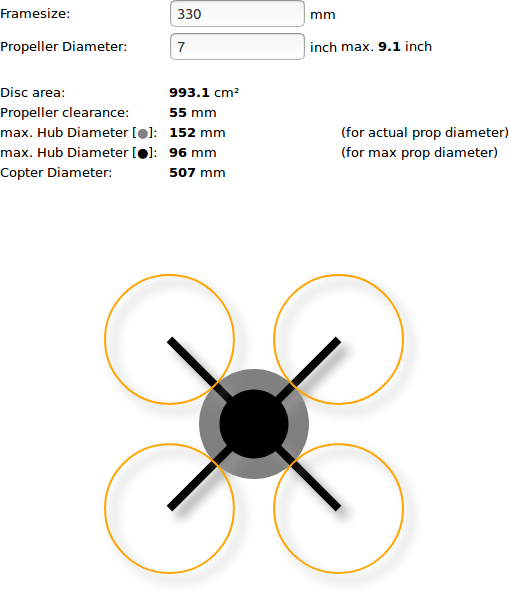
\includegraphics[width=.5\linewidth]{design/330_7.png}
            \caption{First choice of frame}
            \label{fig:330_7}
        \end{figure}
        
        \begin{figure}[!ht]
            \centering
            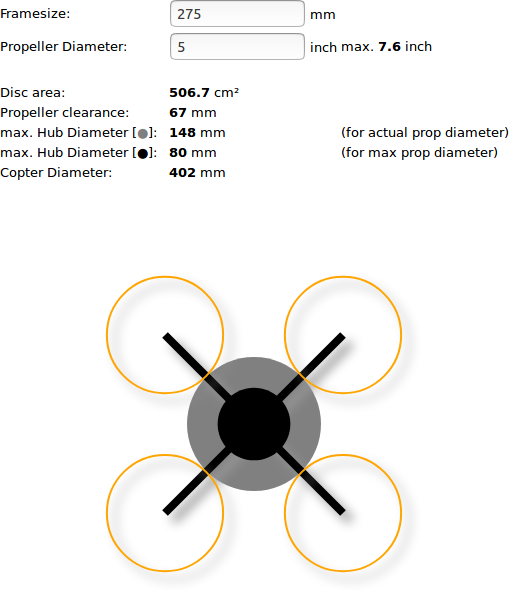
\includegraphics[width=.5\linewidth]{design/275_5.png}
            \caption{Second choice of frame}
            \label{fig:275_5.png}
        \end{figure}
        
        Three frame have been selected from these criteria a 330mm frame (\hyperref[fig:f330]{F330}) and two 275mm frame (\hyperref[fig:minibiggerracer]{Minibigger Racer} and \hyperref[fig:f2mito]{F2 Mito}).
    
        \begin{figure}[!ht]
            \centering
            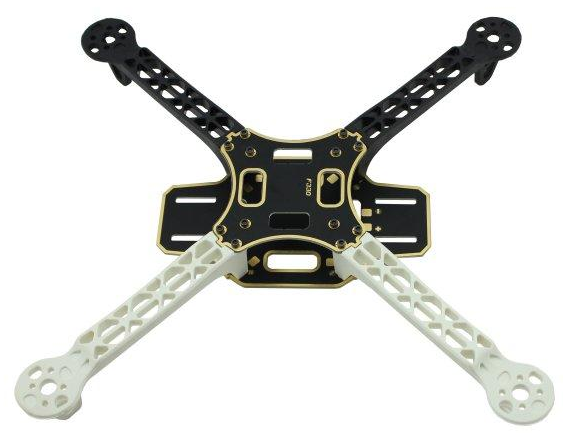
\includegraphics[width=.5\linewidth]{design/f330.png}
            \caption{\href{https://www.banggood.com/DJI-F330-4-Axis-RC-Quadcopter-Frame-Kit-Support-KK-MK-MWC-p-943370.html?rmmds=search&ID=48074&cur_warehouse=CN}{F330}}
            \label{fig:f330}
        \end{figure}
    
        \begin{figure}[!ht]
            \centering
            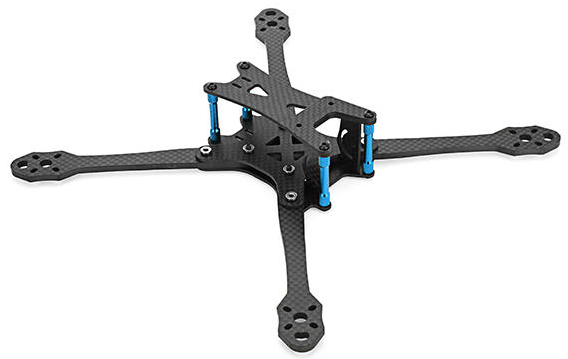
\includegraphics[width=.5\linewidth]{design/minibigger_racer.png}
            \caption{\href{https://www.banggood.com/Minibigger-Racer-255mm-275mm-Carbon-Fiber-4mm-Arm-RC-Drone-FPV-Racing-Frame-Kit-with-Wrench-Tools-p-1241634.html?rmmds=search&ID=228532758&cur_warehouse=CN}{Minibigger Racer}}
            \label{fig:minibiggerracer}
        \end{figure}
        
        \begin{figure}[!ht]
            \centering
            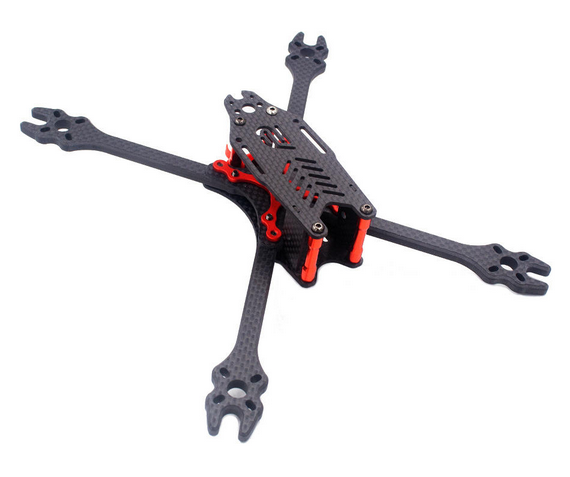
\includegraphics[width=.5\linewidth]{design/f2_mito.png}
            \caption{\href{https://www.banggood.com/F2-Mito-GS-Carbon-Fiber-195220250275mm-Freestyle-Stretch-X-Frame-Kit-for-RC-FPV-Racing-Drone-p-1319168.html?rmmds=search&ID=532758&cur_warehouse=CN}{F2 Mito}}
            \label{fig:f2mito}
        \end{figure}
    
    \section{Propellers}
        The propellers have three major characteristics. Their size, their pitch, and their number of blades.
        
        The size of the propellers have been fixed by the size of the frame.
        
        The higher the pitch the higher the thrust but also the higher the torque needed. So it means more powerful motor. Moreover, the pitch should always be 2/3 of the propeller size because if it is higher it could cause air disturbances (Vortex Ring State). So, the pitch was chosen by taking the highest pitch on the market that respected the 2/3 ratio.
        
        The number of blades impact thrust and efficiency. More blades mean increased thrust but decreased efficiency. As, the drone just a need a thrust-weight ratio of 2, the number of blades chosen is 2.
        
        The propeller specification are generally either \emph{SxPxB} or \emph{SSPPxB}. S being the size, P the pitch and B the number of blades (e.g. for a size of 70mm and pitch of 4.5 and 2 blades, 7x4.5x2 and 7045x2).
        
        For the 330mm frame the propeller chosen was a \hyperref[fig:7045]{propeller 7045} and for the 275mm frame a \hyperref[fig:5030]{propeller 5030}.
    
        \begin{figure}[!ht]
            \centering
            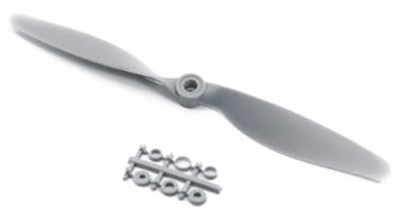
\includegraphics[width=.5\linewidth]{design/7045.png}
            \caption{\href{https://www.banggood.com/Style-7050-7x5-DD-Direct-Drive-Propeller-Blade-CW-CCW-For-RC-Airplane-p-1045332.html?rmmds=search&ID=45905&cur_warehouse=CN}{Propeller 7045}}
            \label{fig:7045}
        \end{figure}
        
        \begin{figure}[!ht]
            \centering
            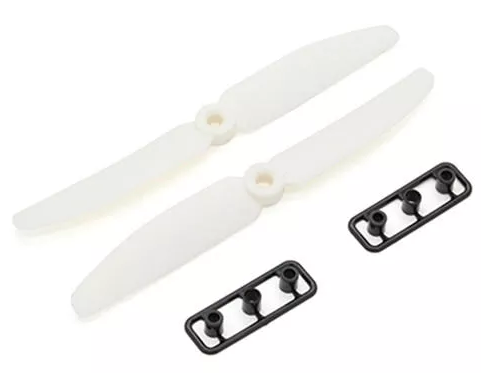
\includegraphics[width=.5\linewidth]{design/5030.png}
            \caption{\href{https://www.banggood.com/2pcs-WSX-5030-53-Inch-ABS-Propeller-White-CWCCW-for-RC-Drone-FPV-Racing-Multirotors-p-1387499.html?rmmds=search&cur_warehouse=CN}{Propeller 5030}}
            \label{fig:5030}
        \end{figure}
        
    \section{Motors}
        The motors have different characteristics. Its width, height and KV.
        
        The width of the motor in our case will be 22mm
        
        Propeller adapter
        
    \section{Battery}
    
    \section{Power Distribution Board}
    
    \section{Flight Controller}
    
    \section{Radio Transmitter/Receiver}
    
    \section{Miscellaneous}
    
    \section{Weight}
        \centering
        \begin{tabular}{cccc}
            Components & Quantities & Weight & Total \\
            Frame & 1 & 150g & 150g \\
            Propeller & 4 & 5g & 20g \\
            Motor & 4 & 30g & 120g \\
            Battery & 1 & 50g & 50g \\
            PDB 
        \end{tabular}